\documentclass[11pt]{article}\usepackage[]{graphicx}\usepackage[]{color}
% maxwidth is the original width if it is less than linewidth
% otherwise use linewidth (to make sure the graphics do not exceed the margin)
\makeatletter
\def\maxwidth{ %
  \ifdim\Gin@nat@width>\linewidth
    \linewidth
  \else
    \Gin@nat@width
  \fi
}
\makeatother

\definecolor{fgcolor}{rgb}{0.345, 0.345, 0.345}
\newcommand{\hlnum}[1]{\textcolor[rgb]{0.686,0.059,0.569}{#1}}%
\newcommand{\hlstr}[1]{\textcolor[rgb]{0.192,0.494,0.8}{#1}}%
\newcommand{\hlcom}[1]{\textcolor[rgb]{0.678,0.584,0.686}{\textit{#1}}}%
\newcommand{\hlopt}[1]{\textcolor[rgb]{0,0,0}{#1}}%
\newcommand{\hlstd}[1]{\textcolor[rgb]{0.345,0.345,0.345}{#1}}%
\newcommand{\hlkwa}[1]{\textcolor[rgb]{0.161,0.373,0.58}{\textbf{#1}}}%
\newcommand{\hlkwb}[1]{\textcolor[rgb]{0.69,0.353,0.396}{#1}}%
\newcommand{\hlkwc}[1]{\textcolor[rgb]{0.333,0.667,0.333}{#1}}%
\newcommand{\hlkwd}[1]{\textcolor[rgb]{0.737,0.353,0.396}{\textbf{#1}}}%
\let\hlipl\hlkwb

\usepackage{framed}
\makeatletter
\newenvironment{kframe}{%
 \def\at@end@of@kframe{}%
 \ifinner\ifhmode%
  \def\at@end@of@kframe{\end{minipage}}%
  \begin{minipage}{\columnwidth}%
 \fi\fi%
 \def\FrameCommand##1{\hskip\@totalleftmargin \hskip-\fboxsep
 \colorbox{shadecolor}{##1}\hskip-\fboxsep
     % There is no \\@totalrightmargin, so:
     \hskip-\linewidth \hskip-\@totalleftmargin \hskip\columnwidth}%
 \MakeFramed {\advance\hsize-\width
   \@totalleftmargin\z@ \linewidth\hsize
   \@setminipage}}%
 {\par\unskip\endMakeFramed%
 \at@end@of@kframe}
\makeatother

\definecolor{shadecolor}{rgb}{.97, .97, .97}
\definecolor{messagecolor}{rgb}{0, 0, 0}
\definecolor{warningcolor}{rgb}{1, 0, 1}
\definecolor{errorcolor}{rgb}{1, 0, 0}
\newenvironment{knitrout}{}{} % an empty environment to be redefined in TeX

\usepackage{alltt}
\title{Sample Report}
\author{Robert I. Kabacoff, Ph.D.}
\usepackage{float}
\usepackage[top=.5in, bottom=.5in, left=1in, right=1in]{geometry}
\IfFileExists{upquote.sty}{\usepackage{upquote}}{}
\begin{document}
\maketitle



\section{Results}

Cholesterol reduction was assessed in a study 
that randomized 50 patients 
to one of 5 treatments. 
Summary statistics are provided in 
Table \ref{table:descriptives}.

% latex table generated in R 3.6.3 by xtable 1.8-4 package
% Tue Dec 08 23:28:09 2020
\begin{table}[ht]
\centering
\caption{Descriptive statistics 
for each treatment group} 
\label{table:descriptives}
\begin{tabular}{lrrr}
  \hline
Treatment & N & Mean & SD \\ 
  \hline
1time &  10 & 5.78 & 2.88 \\ 
  2times &  10 & 9.22 & 3.48 \\ 
  4times &  10 & 12.37 & 2.92 \\ 
  drugD &  10 & 15.36 & 3.45 \\ 
  drugE &  10 & 20.95 & 3.35 \\ 
   \hline
\end{tabular}
\end{table}


The analysis of variance is provided in Table \ref{table:anova}.

% latex table generated in R 3.6.3 by xtable 1.8-4 package
% Tue Dec 08 23:28:09 2020
\begin{table}[ht]
\centering
\caption{Analysis of variance} 
\label{table:anova}
\begin{tabular}{lrrrrr}
  \hline
 & Df & Sum Sq & Mean Sq & F value & Pr($>$F) \\ 
  \hline
trt & 4 & 1351.37 & 337.84 & 32.43 & 0.0000 \\ 
  Residuals & 45 & 468.75 & 10.42 &  &  \\ 
   \hline
\end{tabular}
\end{table}


\noindent and group differences are plotted in Figure \ref{figure:tukey}.

\begin{figure}[H]\label{figure:tukey}
\begin{center}

\begin{knitrout}
\definecolor{shadecolor}{rgb}{0.969, 0.969, 0.969}\color{fgcolor}
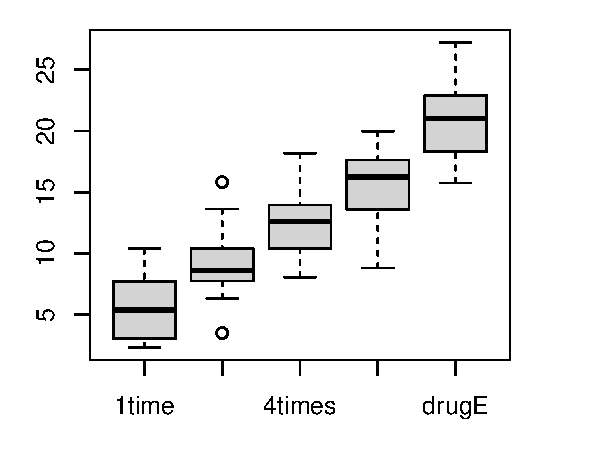
\includegraphics[width=\maxwidth]{figure/unnamed-chunk-4-1} 

\end{knitrout}

\caption{Distribution of response times by treatment.}
\end{center}
\end{figure}
\end{document}
